\section{Latex Examples \label{Latex Examples} }

The pipeline is divided in the following sections:
\begin{itemize} 
   \item  Data Acquisition
   \item  Feature Extraction
   \item  Training Model
   \item  Testing Model
   \item  Visualizing Model
   \item  Deploying Model
\end{itemize} 

At Data Acquisition a robot will be launched in an unknown environment starting to record sensor input. To decrease the amount of unecessary data, the data is recorded in a specific way. The controller will check if there is a safe
passage to a nearby obstacle and then move towards the object on a straight line while recording laser, positional and camera input. This allows to relate, recorded camera inputs at every position along the straight line, with laser data recorded at the same time and with laser data recorded at future instances along the straight line. Every instance along the straight line represents one camera input and a set of laser signals from the image's current
position to the goal. If the image is recorded 2 meter from the obstacle, all subsequent laser recordings will be related to that image and therfore serve as supervisory signal for that instance.\\




The goal of this project is the development of an obstacle avoidcance algorithm, based on self supervised learning, implemented within a ROS environment. As the input are images from a camera, a convolutional neural network is used to train a model, which can then be used to predict produce probabilities about obstacles in front of the cameras field. The data for training like the ground truth labels, shall be collected and processed fully autonomous. This kind of data generation is called self supervised learning.\\

The algorithm is mainly tested and hardened, in a simulation environment, implemented with as less as possible dependencies for the simulation in order to test it as well on a real robot if time and cirumstances allow. Gazebo is used as the simulation environment and the robot selected for this simulation is called TIAGo. TIAGo was chosen, as the university has a real world model of this robot in its laboratory. TIAGo has also the necessary camera and a laser scanner, which will be used to produce the ground truth labes related to the camera input.\\

In the first step, the data necessary to create a dataset, is obtained fully autonomous via the sensors. The sensors used for this project, are the the camera, a laser scanner and odometry input. To increase the quality of the dataset, the controller to collect the data will use a similar approach like described in \cite{nava2019learning} .\\

In the second step, the stored sensor data is converted into a specific format required for training the neural network. Here, at any time t of a sensor, the corresponding data of the other sensors need to be connected in order. To compare different models with each other, different suggestions from other projects can be implemented. For the training of the neural network, the camera data should be used as input and the laser data as output. The laser will be limited to 5 ranges and a limited distance will be considered as valid. The return values are considered as binary ground truth labels and indicate whether an object is located in the immediate vicinity or not. In order to establish an efficient connection between the camera and the laser data, various implementations can be used here, which are discussed later in detail in section x.\\ 

After the dataset is generated, the next step is to implement the training and evaluation of the model. Since the input data are 2-dimensional images, a convolutional neural network will be created for this project. By varying the parameters, as well as by different ways of generating the dataset, different models can be created and tested against each other after deployment.\\

In the last step, after deployment of the model has been taken place, it can be tested and  compared for its efficiency with other models. The last two steps, or even the first and second, can be run through several times to document different results.


%\subsection{Problem Definition \label{Problem Definition} } 

Ein g��eres Dokument\footnote{Fu�noten sind ebenfalls problemlos m�glich.} zerlegt man am besten in ein "'Zentral-Dokument"' und die
einzelnen Kapitel bzw. Abschnitte (s.~Datei {\code Thesis.tex}. Der \LaTeX\
"'Source Code"' wird �bersetzt in das DVI-Format. Das DVI-File kann dann auf dem
Bildschirm angezeigt und/oder gedruckt werden oder in ein anderes Format gewandelt
werden (\zb PostScript, PDF, HTML).

Befehle (Bsp.):
\begin{verbatim}
> latex Thesis.tex
> dvips Thesis.dvi 
> dvipdf Thesis.dvi
> ghostview Thesis.ps 
> ps2pdf Thesis.ps Thesis.pdf 
> latex2html Thesis.tex 
\end{verbatim} 

Alternativ kann der \LaTeX\ "'Source Code"' (ohne Umwege �ber das DVI-Format) direkt in das PDF-Format �bersetzt werden:
\begin{verbatim}
> pdflatex Thesis.tex
\end{verbatim} 

Das Literaturverzeichnis erstellt man am besten mit dem Programm
BibTeX. Voraussetzung ist nat�rlich, dass man eine BibTex-Datei mit den
Literatur-Eintr�gen erstellt hat (in diesem Fall: Literatur.bib). 
\begin{verbatim}
> latex Thesis.tex
> bibtex Thesis
> latex Thesis.tex
> latex Thesis.tex
\end{verbatim} 

Hier folgen noch ein paar Beispiele f�r \LaTeX-Konstruktionen bzw.\ selbst definierte
Kommandos Kommandos Kommandos Kommandos Kommandos: 

\paragraph{Querverweis:} Dies ist ein Querverweis auf \secref{Zielsetzung} (das Kommando
\verb+\secref{}+ ist von mir in {\code Abkuerzugen.tex} definiert). 

\paragraph{Literaturhinweise:} Ein Literaturhinweis
entsteht durch \cite{mandl99} bzw. durch \cite{sing00, zeller02,edwards00}. Das
Kommando \verb+\cite{...}+ ist bereits in \LaTeX\ definiert. Die Quellen-Angaben
schreiben Sie in eine Datei mit der Endung \verb+.bib+, n�heres s.~Tutorial. 

Die verschiedenen Kommandos in der Datei {\code Abkuerzugen.tex} \mymargin{nur am
Rande, bei Bedarf} ergeben \ua folgende Abk�rzungen; \ia und \zb und \dht und \zz
sowie eine Randbemerkung.

\begin{itemize} 
   \item  eine Aufz�hlung
   \item  noch ein Punkt 
   \item  bla
\end{itemize} 
\LaTeX und Emacs: Abk�rzungen machen das Leben leichter. Einige Definitionen finden
sich in der Datei {\code Abkuerzugen.emacs}. So bewirkt \zb die Eingabe von
\verb+bgit<space>+, dass Emacs die folgenden drei Zeilen einf�gt: 
\begin{verbatim}
\begin{itemize} 
   \item 
\end{itemize}  
\end{verbatim} 
Die Datei {\code Abkuerzugen.emacss} muss von Emacs geladen
werden, am besten automatisch durch einen Eintrag in {\code .emacs},{\code
  .gnu-emacs} oder{\code .gnu-emacs-custom} je nach Installation \smiley.
\begin{verbatim} 
  (if (file-readable-p "~/etc/TeX/Abkuerzugen.emacs")
      (read-abbrev-file "~/etc/TeX/Abkuerzugen.emacs")) 
\end{verbatim} 

bla bla bla bla bla bla bla bla bla bla bla bla bla bla bla bla bla
bla bla bla bla bla bla bla bla bla bla bla bla bla bla bla bla bla
bla bla bla bla bla bla bla bla bla bla bla bla bla bla bla bla bla
\begin{enumerate} 
   \item  eine Aufz�hlung nummeriert 
   \item  Aufz�hlungen k�nnen auch geschachtelt werden \ldots
   \item  bla
\end{enumerate} 

bla bla bla bla bla bla bla bla bla bla bla bla bla bla bla bla bla
bla bla bla bla bla bla bla bla bla bla bla bla bla bla bla bla bla
bla bla bla bla bla bla bla bla bla bla bla bla bla bla bla bla bla
bla bla bla bla bla bla bla bla bla bla bla bla bla bla bla bla bla

\begin{table}[htb] 
\caption{Eine Tabelle hat (manchmal) eine �berschrift} 
\begin{center}
\begin{tabular}{|rc|}           \hline
eine Tabelle & zweite Spalte \\ \hline \hline 
  a          & b             \\ 
  ccc        & ddd           \\ 
 aber        & ohne          \\ 
 Buch        & geht's nicht  \\ \hline 
\end{tabular} 
\end{center}
\end{table} 

bla bla bla bla bla bla bla bla bla bla bla bla bla bla bla bla bla
bla bla bla bla bla  


%\subsection{Objectives \label{Objectives} } 

bla bla bla bla bla bla bla bla bla bla bla bla bla bla bla bla bla
bla bla bla bla bla bla bla bla bla bla bla bla bla bla bla bla bla
bla bla bla bla bla bla bla bla bla bla bla bla bla bla bla bla bla

\begin{figure}[htbp]
\centering 
 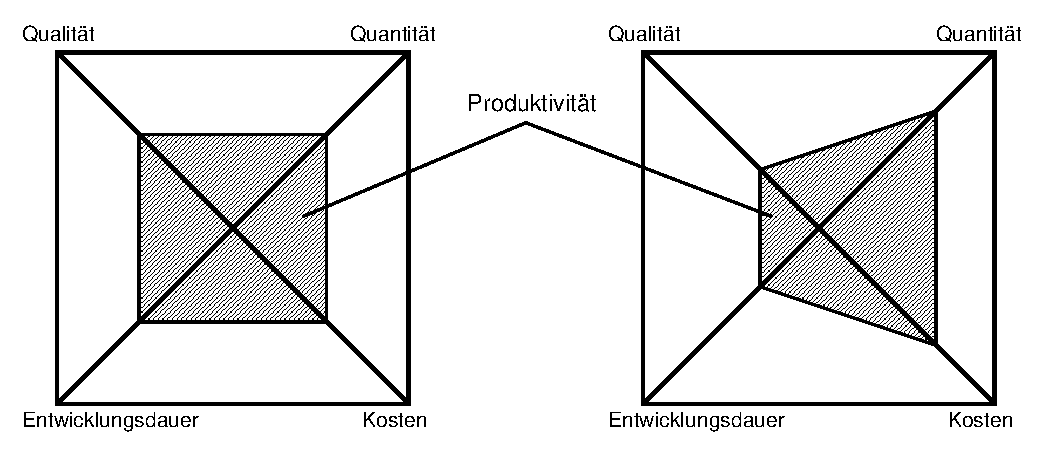
\includegraphics[width=0.8\textwidth]{Bilder/magicSquare} 
 \caption{Das magische Quadrat der konkurrierenden Ziele (als encapsulated
          postscript)  \label{magicSquare}}
\end{figure}
Auf Abbildungen kann nat�rlich auch referenziert werden \zb durch
"'\figref{magicSquare} auf Seite~\pageref{magicSquare}"'. Dies setzt allerdings
voraus, dass man ein Label definiert hat (\zb \verb+\label{magicSquare}+). Der Befehl
\verb+\figref{..}+ ist nicht von \LaTeX\ definiert sondern in der Datei {\code
Abkuerzugen.tex}.  Hier sieht man auch, wie man Anf�hrungszeichen schreibt \ldots
  
bla bla bla bla bla bla bla bla bla bla bla bla bla bla bla bla bla
bla bla bla bla bla bla bla bla bla bla bla bla bla bla bla bla bla
bla bla bla bla bla  

\newpage
%\subsection{Noch ein paar Anmerkungen \label{Anmerkungen}} 

bla bla bla bla bla bla bla bla bla bla bla bla bla bla bla bla bla
bla bla bla bla bla bla bla bla bla bla bla bla bla bla bla bla bla

\begin{comment} 
\cbstart 
\ \vspace{0.5ex}
\hrule 
\ \vspace{0.5ex}

Dieser Abschnitt erscheint nur, wenn der Befehl \verb+\includecomment{comment}+ in
der \LaTeX -Hauptdatei steht.  Mit einem \verb+%+ -Zeichen kann er auskommentiert
werden. Dann verschwindet dieser Absatz aus dem Dokument.

Kommentar-Bereiche sind praktisch um Textteile im Dokument "'parken"' zu k�nnen. Bei
Bedarf kann man die Teile sichtbar bzw.\ unsichtbar schalten.  Der graue Balken am
Rand wird durch die Befehle \verb+\cbstart+ und \verb+\cbend+ erzeugt. Dazu muss das
Package \verb+changebar+ geladen werden. 
\ \vspace{0.5ex}
\hrule 
\ \vspace{0.5ex}\cbend
\end{comment} 

bla bla bla bla bla bla\footnote{Fu�noten sind ebenfalls problemlos m�glich.} bla bla
bla bla bla bla bla bla bla bla bla bla bla bla bla bla bla bla bla bla bla bla bla
bla bla bla bla bla bla bla bla bla bla bla bla bla bla bla bla bla bla bla bla bla
bla bla bla bla bla bla



